\section{Algorithm execution}
\label{sec-algorithm-execution}

\textbf{Created by:} Milos Drobnjakovic \\
\textbf{Modified by:} Milos Drobnjakovic \\

\subsection*{Scenario Objective}


This scenario demonstrates how to represent the execution of algorithms within the context of the \textbf{BFO/IOF ontology}. It specifically addresses cases where algorithm executions generate \textbf{Information Content Entities (ICEs)} as outputs. Algorithms that do not produce outputs are beyond the scope of this pattern.

\subsection*{Key Points}
\begin{itemize}
    \item This pattern is intended for algorithms integrated into a software system.
    \item Only algorithm executions resulting in ICEs are covered; executions without outputs are excluded.
\end{itemize}


\subsection*{General Pattern Description}
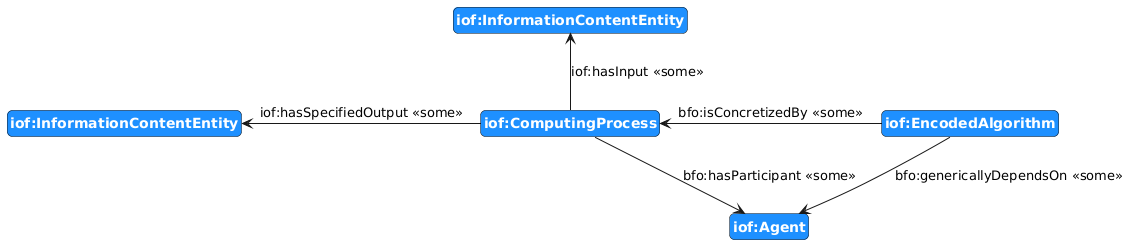
\includegraphics[scale=0.6]{scenarios/algorithm-execution/images/algorithm-execution-general.png}

...

\subsubsection*{Use Case: Drill failure prediction} 
A multilayer perceptron (MLP – a type of a neural network) is used to predict drill failure based on five measured parameters: ‘tool wear’, ‘air temperature’, ‘process temperature’, ‘torque’,’rotational speed’. The model uses the given parameters and outputs either ‘FAIL’ or ‘NOT FAIL’.

\subsubsection*{Use-Case Pattern Description}

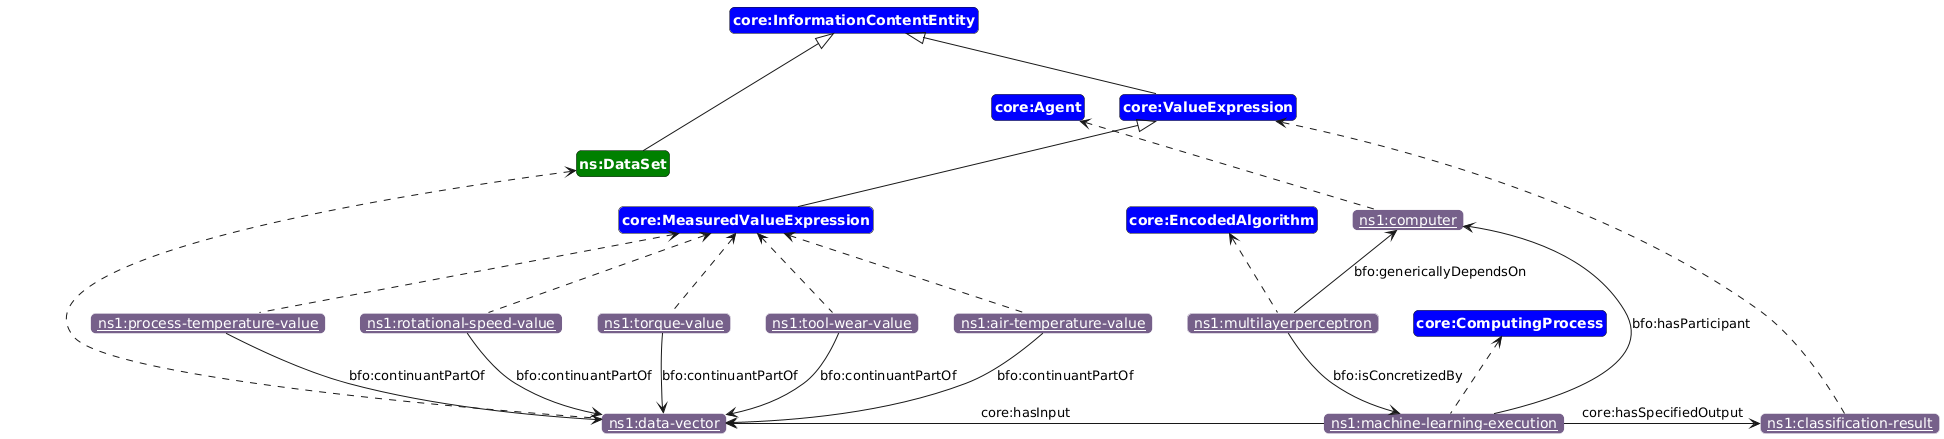
\includegraphics[scale=0.23]{scenarios/algorithm-execution/images/algorithm-execution-usecase1.png}
This use case illustrates the execution of a machine learning model, \texttt{mutltilayerperceptron}, on a computer system. The model is an instance of \texttt{Encoded Algorithm} and is \texttt{concretized} through a \texttt{Computing Process} representing its execution.

\subsection*{Actors and Dependencies}  
\begin{itemize}
    \item The \texttt{mutltilayerperceptron}  \texttt{generically depends on} a \texttt{computer} (an instance of \texttt{Agent}) that \texttt{participates in} the \texttt{machine-learning-execution} (an instance of \texttt{ComputingProcess}.
    \item M\texttt{machine-learning-execution} relies on (\texttt{hasInput}) measured values associated with the drill and the drilling process as input data (represented as various instances of \texttt{MeasuredValueExpression}.
\end{itemize}

\subsection*{Process and Output}  
\begin{itemize}
    \item The model execution produces (\texttt{has-specified-output}) a \texttt{classification-result}, an instance of \texttt{ValueExpression}.
    \item The \texttt{classification-result} can take one of two possible values, represented by the \texttt{hasSimpleExpressionValue} property:
    \begin{enumerate}
        \item \texttt{NOT-FAILURE}
        \item \texttt{FAILURE}
    \end{enumerate}
\end{itemize}

\subsection*{Diagram Context}  
The diagram below demonstrates a specific example where the \texttt{classification-result} has the value \texttt{NOT-FAILURE}. For simplicity:
\begin{itemize}
    \item The actual measurement values and their units are excluded from the diagram.
    \item Associations between measured values and entities such as “drill attributes” or the “drilling process” are not shown.
\end{itemize}

\subsection*{Further Guidance}  
For details on connecting measured values with their respective entities, please refer to the \href{placeholder link}{detailed guide}.  

\subsubsection*{Use-Case Example Data}

For this use case a publicly available dataset was used: Predictive Maintenance⚙️ 

The dataset is a single CSV table consisting of the columns: ‘tool wear’, ‘air temperature’, ‘process temperature’, ‘torque’,’rotational speed’, ‘type’ and ‘product ID’, ‘failure type’.

\begin{tabularx}{\textwidth}{|l|X|X|X|X|X|X|X|X|X|X|}
\hline
Product ID & Type & Air temperature {[}K{]} & Process temperature {[}K{]} & Rotational speed {[}rpm{]} & Torque {[}Nm{]} & Tool wear {[}min{]} & Target & Failure Type \\ \hline
M14860     & M    & 298.1                   & 308.6                       & 1551                       & 42.8            & 0                   & 0      & No Failure   \\
L47181     & L    & 298.2                   & 308.7                       & 1408                       & 46.3            & 3                   & 0      & No Failure   \\
L47182     & L    & 298.1                   & 308.5                       & 1498                       & 49.4            & 5                   & 0      & No Failure   \\ \hline
\end{tabularx}

For prediction purposes, type and Product ID are omitted and are as such not included in the RDF. The model outputs the entries of the  target column which is then converted to 'No-failure' or 'Failure'. For brevity, conversion of target to failure type is omitted.
\subsubsection*{Data Mapping Description}

\begin{verbatim}
INSERT DATA {
  ns-1:air-temperature-value a iof-core:MeasuredValueExpression ;
    bfo:continuantPartOf ns-1:data-vector-1 .
  ns-1:process-temperature-value a iof-core:MeasuredValueExpression ;
    bfo:continuantPartOf ns-1:data-vector-1 .
  ns-1:tool-wear-value a iof-core:MeasuredValueExpression ;
    bfo:continuantPartOf ns-1:data-vector-1 .
  ns-1:torque-value a iof-core:MeasuredValueExpression ;
    bfo:continuantPartOf ns-1:data-vector-1 .
  ns-1:rotational-speed-value a iof-core:MeasuredValueExpression ;
    bfo:continuantPartOf ns-1:data-vector-1 .
  ns-1:data-vector-1 a ns-1:DataSet .
  ns-1:DataSet rdfs:subClassOf iof-core:InformationContentEntity .
  ns-1:machine-learning-execution a iof-core:ComputingProcess ;
    iof-core:hasInput ns-1:data-vector-1 ;
    iof-core:hasSpecifiedOutput ns-1:classification-result ;
    bfo:hasParticipant ns-1:computer .
  ns-1:classification-result a iof-core:ValueExpression .
  ns-1:computer a iof-core:Agent .
  ns-1:multilayerperceptron a iof-core:EncodedAlgorithm ;
    bfo:isConcretizedBy ns-1:machine-learning-execution ;
    bfo:genericallyDependsOn ns-1:computer .
}
\end{verbatim}

\subsubsection*{Data Validation}

\begin{verbatim}
# Shape for MeasuredValueExpression
ns-1:MeasuredValueExpressionShape a sh:NodeShape ;
    sh:targetClass iof-core:MeasuredValueExpression ;
    sh:property [
        sh:path bfo:continuantPartOf ;
        sh:class ns-1:DataSet ;
        sh:nodeKind sh:IRI ;
        sh:message "Each MeasuredValueExpression must be part of a DataSet." ;
    ] .

# Shape for ComputingProcess
ns-1:ComputingProcessShape a sh:NodeShape ;
    sh:targetClass iof-core:ComputingProcess ;
    sh:property [
        sh:path iof-core:hasInput ;
        sh:class ns-1:DataSet ;
        sh:nodeKind sh:IRI ;
        sh:message "ComputingProcess must have an input of type DataSet." ;
    ] ;
    sh:property [
        sh:path iof-core:hasSpecifiedOutput ;
        sh:class iof-core:ValueExpression ;
        sh:nodeKind sh:IRI ;
        sh:message "ComputingProcess must have an output of type ValueExpression." ;
    ] ;
    sh:property [
        sh:path bfo:hasParticipant ;
        sh:class iof-core:Agent ;
        sh:nodeKind sh:IRI ;
        sh:message "ComputingProcess must have a participant of type Agent." ;
    ] .

# Shape for EncodedAlgorithm
ns-1:EncodedAlgorithmShape a sh:NodeShape ;
    sh:targetClass iof-core:EncodedAlgorithm ;
    sh:property [
        sh:path bfo:isConcretizedBy ;
        sh:class iof-core:ComputingProcess ;
        sh:nodeKind sh:IRI ;
        sh:message "EncodedAlgorithm must be concretized by a ComputingProcess." ;
    ] ;
    sh:property [
        sh:path bfo:genericallyDependsOn ;
        sh:class iof-core:Agent ;
        sh:nodeKind sh:IRI ;
        sh:message "EncodedAlgorithm must generically depend on an Agent." ;
    ] .
\end{verbatim}

